\section{Sơ bộ}
\subsection{Tính chất của đồ thị con và đồ thị phân chia}

\begin{corollary}
    Đồ thị con của đồ thị phẳng là đồ thị phẳng
\end{corollary}

\begin{proof}
    Nếu $G$ là đồ thị phẳng, nghĩa là tồn tại một biểu diễn phẳng của $G$. Với mọi đồ thị con
    $H$ của $G$, ta có thể tìm đươc các đỉnh và cạnh của $H$ trong biểu diễn phẳng của $G$.
    Từ đó, ta dựng được một biểu diễn phẳng của $H$.
\end{proof}


\begin{corollary}
    Đồ thị phân chia của một đồ thị không phẳng là một đồ thị không phẳng.
\end{corollary}
\begin{proof}
    Giả sử đồ thị không phẳng $G$ có một đồ thị phân chia $G'$ của $G$ là đồ thị phẳng.
    Khi đảo ngược phép \hyperref[def:subdivision]{\textit{chia nhỏ}}, ta thu được đồ thị $G$ cũng là đồ thị phẳng, mâu thuẫn.
    Vậy nên, nếu $G$ không phẳng thì $G'$ cũng không phẳng.
\end{proof}

\subsection{Tính chất đồ thị 2-Connected}
\begin{corollary}
    Xóa một đỉnh khỏi đồ thị 2-liên thông không làm mất tính liên thông của nó.
\end{corollary}
\begin{proof}
    Vì đồ thị $G$ là 2-liên thông nên $\kappa(G) \geq 2$. Nếu việc loại bỏ 1 điểm khỏi $G$ làm nó mất tính liên thông nghĩa là $\kappa(G) \leq 1$. Vô lý.
\end{proof}

\begin{corollary}
    Mọi cặp đỉnh trong đồ thị 2-connected đều cùng nằm trên một chu trình.
    \begin{proof}
        Quy nạp:

        Trường hợp cơ bản: $u$ kề $v$
        \begin{center}
            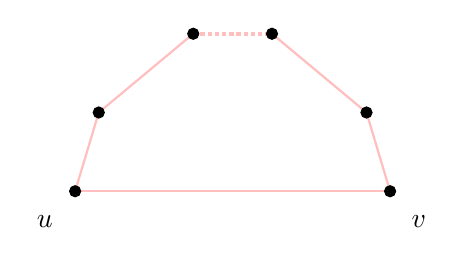
\begin{tikzpicture}
                \draw[pink, thick] (0,0) -- (0.3,1);
                \draw[pink, thick] (0.3,1) -- (1.5,2);
                \draw[densely dotted, pink, ultra thick] (1.5,2) -- (2.5,2);
                \draw[pink, thick] (2.5,2) -- (3.7,1);
                \draw[pink, thick] (3.7,1) -- (4,0);
                \draw[pink, thick] (0,0) -- (4,0);
                \node at (0,0,1) {$u$};
                \node at (4.75,0,1) {$v$};
                \filldraw[black] (0,0) circle (2pt);
                \filldraw[black] (0.3,1) circle (2pt);
                \filldraw[black] (1.5,2) circle (2pt);
                \filldraw[black] (2.5,2) circle (2pt);
                \filldraw[black] (3.7,1) circle (2pt);
                \filldraw[black] (4,0) circle (2pt);
            \end{tikzpicture}
        \end{center}
        Quy nạp: $u,v$ có khoảng cách $d+1$
        \begin{center}
            \begin{tikzpicture}
                \draw[pink, thick] (0,0) -- (0.3,1);
                \draw[pink, thick] (0.3,1) -- (1.5,2);
                \draw[densely dotted, pink, ultra thick] (1.5,2) -- (2.5,2);
                \draw[pink, thick] (2.5,2) -- (3.7,1);
                \draw[pink, thick] (3.7,1) -- (4,0);
                \draw[pink, thick] (0,0) -- (2,0);
                \draw[black, thick] (3,0) -- (4,0);
                \draw[pink, thick] (4,0) -- (5,0);
                \draw[densely dotted, black, ultra thick] (2,0) -- (3,0);
                \draw[pink, thick] (2.5,0) -- (3.25,-1);
                \draw[pink, thick] (3.35,-1) -- (4.5,-1);
                \draw[pink, thick] (5,0) -- (4.5,-1);
                \draw[pink, thick] (2,0) -- (2.5,0);

                \node at (0,0,1) {$u$};
                \node at (5.75,0,1) {$v$};
                \node at (4.4,0,1) {$w$};
                \filldraw[black] (0,0) circle (2pt);
                \filldraw[black] (0.3,1) circle (2pt);
                \filldraw[black] (1.5,2) circle (2pt);
                \filldraw[black] (2.5,2) circle (2pt);
                \filldraw[black] (3.7,1) circle (2pt);
                \filldraw[black] (1,0) circle (2pt);
                \filldraw[black] (2,0) circle (2pt);
                \filldraw[black] (3,0) circle (2pt);
                \filldraw[black] (4,0) circle (2pt);
                \filldraw[black] (5,0) circle (2pt);
                \filldraw[black] (3.25,-1) circle (2pt);
                \filldraw[black] (4.5,-1) circle (2pt);

                \draw [decorate, decoration = {calligraphic brace, mirror, raise=5pt}] (0,-1.5) --  (4,-1.5) node[pos=0.5,below=10pt,black]{$d$};
            \end{tikzpicture}
        \end{center}
    \end{proof}
\end{corollary}